\section{Proposal}
\label{sec:intro}

%%State of the world
Disaggregated computing promises higher resource density, increased
power-efficiency, and flexible application scalability in datacenters.
While enticing, these benefits have remained mostly untapped (with the
exception of persistent storage) due to the proportionally large
overhead of accessing remote resources. Nowhere is this disparity more
noticeable than remote memory. Separating CPUs last level cache from
their main memory incurs roughly a 20x overhead (approximately
50\textit{ns} to 1\textit{us}).  The cost is only acceptable for
select asynchronous workloads, such as paging out infrequently touched
data~\cite{gms}, but are entirely unrealistic when multiple CPUs
requires consistency for frequent reads and writes to remote memory.
Figure~\ref{fig:overview} illustrates resource placement in a
disaggregated rack in contrast to traditional servers.

Researchers and industry leaders have proposed techniques which reduce
cost of write contention with regard to remote
memory~\cite{aguilera2019designing,cell,sonuma,storm,clover}. A common
goal among them is to provide $O(1)$ read and write costs in the
common case. To achieve this strategy such as memory versioning,
checksums, and memory enforced serialization have been
proposed~\cite{aguilera2019designing}.

%%
%%These are reasons from the proposal
%%
%%These strategies have
%%significant shortcomings in their current implementations: versioning,
%%typically performed by an endhost, requires that a failed remote
%memory write (\textit{RDMA-CAS}) must be propagated back to the writer
%over a network (a full RTT) prior to it reissuing a consistent write.
%Writers also only learn their version is out of date upon failing a
%write, making it a common occurrence as version information ages.
%Serialization at the memory is more tenable, but requires currently
%nonexistent technologies. Specifically it reuqires either a memory
%controller or memory itself to perform a variety of inplace arthemtic
%operations in the absense of a CPU. These instructions are required to
%provide memory versioning for consistancy, and to trigger notification
%messages to alert remote CPU's that a memory address has been dirtied
%by another CPU's write.  We consider an alternative network
%centralized approach which achieves the same benefit of a memory
%centric architecture, with fundamentally lower latency, and currently
%available technology.

%% WORDS
Prior remote memory sysetms require the use of CPU's on remote
machines to coordinate RDMA~\cite{cell,sonuma,storm,erpc,farm}. Remote
CPU's provide RDMA serialization and simplify consistancy for
distributed data structures. Disaggregated memory poses a new problem:
\textit{How can remote memory be coordinated without a remote CPU?}.

%%
Clover is the first attempt to have fast consistent remote memory
without any datapath coordination via remote CPU~\cite{clover}. Other
recent approaches such as Remote Reigons~\cite{reigons} discount
remote consistancy, and HP's the machine requires computation in
remote memory, which relies on non existant
hardware~\cite{aguilera2019designing}.

%%
Clover proposes that disagregated datastructes seperate their
computational concerns into distinct responsibilities. Mainly memory
servers, which passivle accepty RDMA requests, Clients which issues read and
writes to the remote memory banks, and Metadata severs which
centralize and keep consistant the shared metadata of the disagregated
datastructures.

Through their experimentation they find that ideal throughput is
gained by placing client shared metadata out of datapath entirely, and
updating it opprotunistically. Placing a metadata coordinater in the
datapath quickly leads to a performance bottlenck. Their algorithm
concetrates on maximizing read operations, and allows for lockless
line rate reads in the absence of writes. In the presence of writes
however clovers operation throughput decreases due to contention. When
concurrent writes contest the same data a race occurs in which the
fastest writer wins. The slower writer will fail, and is forced to
retry it's write after searching through clovers remote data structure
for the next write location. On write heavy workloads these race
conditions happen frequently~\ref{fig:conflicts}, which leads to a
sharp decrease in overall throughput.

\begin{figure}
    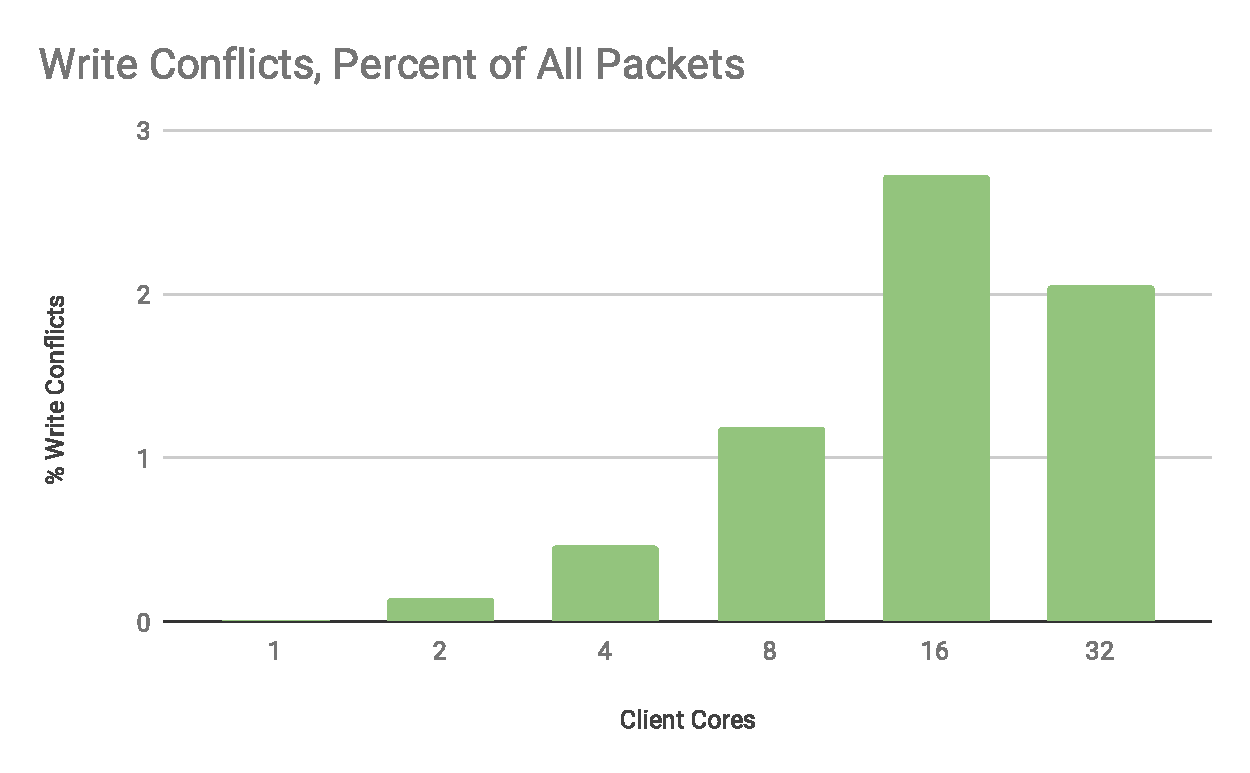
\includegraphics[width=0.45\textwidth]{fig/write_conflicts.pdf}
    \caption{Clover write conflicts grow with the number of clients
    (50\% write zipf 0.99 distribution)}
    \label{fig:conflicts}
\end{figure}


%% what are we discussing
Clover's write strategy is opprotunistc, in that it attempts to make
multiple updates without aquiring locks, in the hope that no conflicts
occur. When they do occur it's just job of the writer to reconcile the
conflict. This opprotunism amortizes the cost of lock aquisition when
contention is low, providing average case O(1) read/write and is used
in many high throughput concurrent datastructures.\todo{cite cocurrent
data structures}.

%%
We propose a middleground betwen prior centralized approaches, and
clover's out of datapath metadata separation. Our insite is that by
caching small ammount of a disaggregated data structures metadata in a
centralized location, write conflicts can be resolved in the data path
allowing for conflict free full read and write throughput of
disaggregated data structures.

%%
Using Clover as a platform to prove our concept we design a
ligthweight middle box algorithm which intercepts clovers RDMA read
and write requets, caches a small ammount (64 byte per key) ammount of
structural meta data and resolves write conflicts within the data
path. 

%%
Our algorithm is implemented in DPDK, but is designed to have
extremely low space and computational overhead making it ideals for
network devices such as programable switches and NICSs.



%%our position

\begin{figure*}
      \centering
      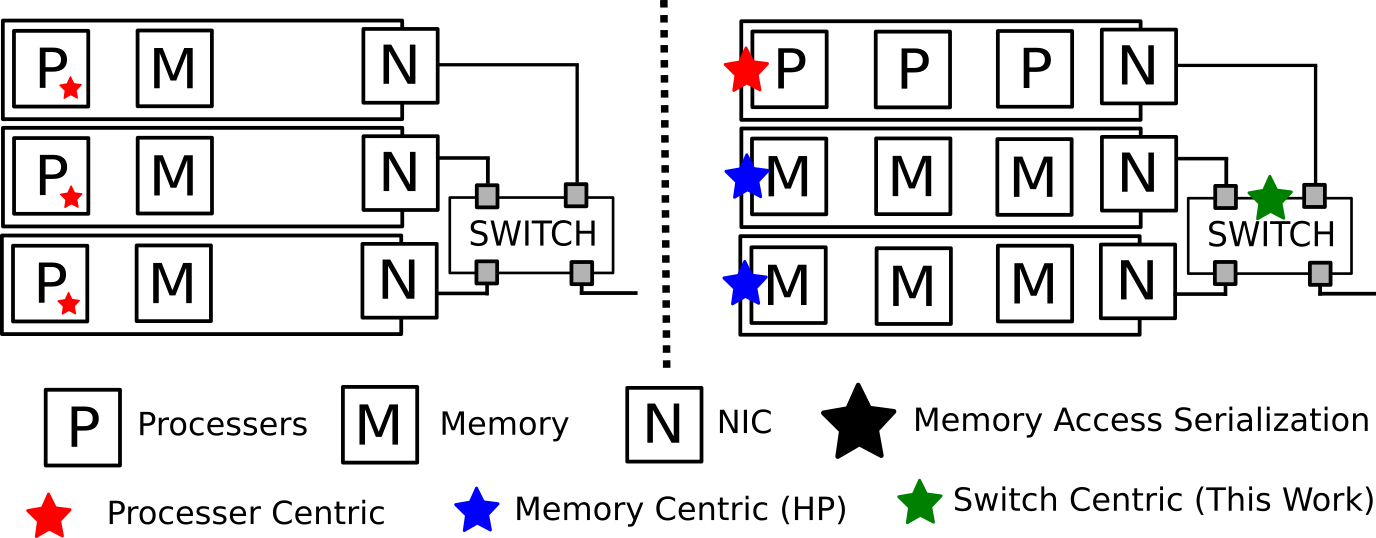
\includegraphics[width=0.95\textwidth]{fig/overview.png}
      %%
      \caption{Anatomy of a disaggregated rack. On the left a
      traditional rack with processors colocated with their memory
      interconnected by a switch. On the right is a high density
      disaggregated rack with processors separated from their memory
      by a top of rack switch. Stars mark locations for memory access
      serialization. Red denotes traditional processor centric
      serialization~\cite{ memc3, cell, sonuma, storm, clover}, blue marks a
      memory centric architecture~\cite{aguilera2019designing}, and
      green marks a switch centric solution similar in spirit to
      proposed middle box solutions~\cite{254120}.
      \label{fig:overview}
      %%
      }
\end{figure*}


This work makes the contention that a programmable switch is an ideal
centralized point at which to implement a remote memory controller.
for rack scale disaggregation.  Prior work has suggested the need for
a distributed memory controller~\cite{254120}. But none have been
built or proposed with existing hardware. We posit that if all remote
reads and writes are performed within a rack using RDMA a programmable
top of rack switch (TOR) will see every memory operation. This fact
allows it to act as a centralized serialization point, where the last
instance of concurrency between the reads and writes of remote CPUs is
the egress port of the switch. The switch can therefore notify CPUs
which contest the same memory regions that their writes have failed
within half an RTT, whereas performing the notify at memory requires a
full RTT. In addition to the fast rejection of out of date writes,
modern programmable switchs \textit{currently} have the ability to
maintain memory version numbers, and to store lists of CPU's which
wish to be notified upon a write occurring to a shared memory location
via a multicast of the write packet. This simple mechanism notifies
CPU's which share a remote region that their local cache is dirty
within half of an RTT of the write being issued.
Figure~\ref{fig:notify} illustrates how switch centric memory
management simplifies a notification protocol. 

%%Struggles
A key problem with using a switch as a memory controller is its
available memory. For context a Barefoot Tofino has 50-100MB of
programmable SRAM. By default this SRAM is used as buffers.
Reallocating buffer memory for storage trades off the usability of a
switch as a packet forwarding device. Therefore any use SRAM for
additional application must be carefully considered. Each shared
region must be bookmarked with a version number, and a list of
\textit{subscriber} CPU's must be maintained.  Maintaining version
numbers for byte addressable memory is unrealistic as the number of
versions would grow with the size of memory, and because a remote read
for a single byte of data is largely impractical. We assume that
remote memory is at least accessed in the form of pages or blocks
(likely 4K) which reduces the number of version numbers which must be
maintained.  Maintaining notify groups is a larger problem as each
shared region requires a list of CPUs with read/write access. As the
number of CPU's grows so too does the per block memory requirement of
the switch.  We place the responsibility of maintaining the read/write
access list to the cores themselves.  Prior to accessing a region a
core must be admitted via con census.  When a write occurs, the
writing node appends the list of cores which share the recon to the
packet. The switch parses the packet for the list and broadcasts the
notify message to the affected cores. While this adds bandwidth
overhead to each write it significantly reduces memory usage on the
switch where resources are tight. Figure~\ref{fig:notify} illustrates
the placement of memory state, alongside a notify algorithm in the
context of 3 distinct resource centric architectures.

\begin{figure*}
      \centering
      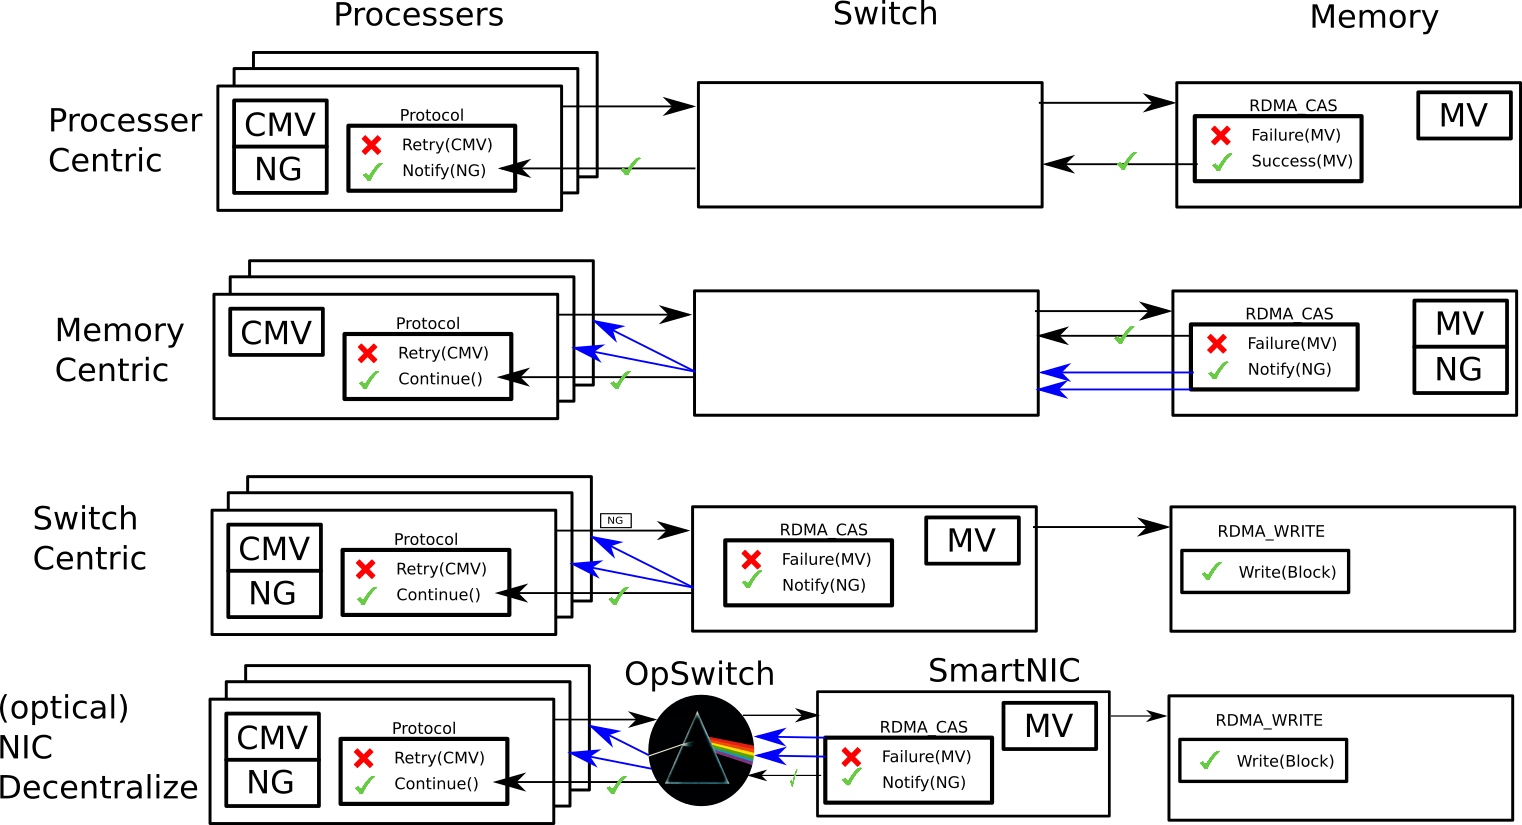
\includegraphics[width=0.95\textwidth]{fig/optical-extension.png}
      %%
      \caption{Illustration of a successful write across different
      resource centric architectures with the location of memory
      consistency information labeled: \textbf{MV} (Memory version),
      \textbf{CMV} (Cached Memory Version) and \textbf{NG} (Notify
      Groups). Processor centric writes are
      initiated and validated by processors exclusively. Successful
      writes require 1 RTT. Notifications, and retries (Not depicted)
    incur additional round trips. A memory centric architecture places
    memory version and notify groups in remote memory. Upon a
    successful write \textit{notify} messages (blue) are set to each
    group member with updated memory versions. Switch centric
    architecture places memory versions, and notification
    responsibility to the switch. Processors send notify group info
    with writes to reduce memory overhead on the switch. Switch
    centric architecture saves half an RTT over memory centric, and
    cuts notify bandwidth in half. In the presence of an optical
    network, with no centralized switching chip, pNICs can provide the
    same functionality for a single server memory bank.
    %%
      \label{fig:notify}
    }
\end{figure*}


%%Position
We consider our use of a programmable switch as a remote memory
controller to be a disaggregation primitive upon which other
disaggregated systems and algorithms can be layered. We expose a
notification API as the lowest level interface with which applications
can utilize the distributed memory controller (\textit{Publish()},
\textit{Subscribe()}). To show it's applicability to existing
disaggregated systems we build both a cache coherent write interface
similar to soNUMA~\cite{sonuma}, and transactional interface upon the
notify API. We port three existing disaggregated systems
Storm~\cite{storm}, Clover~\cite{clover}, and Cell~\cite{cell} and
demonstrate throughput improvements for write intensive workloads
without degrading the performance of reads.


\section{Software and Hardware}

\noindent\textbf{Hardware}
\begin{itemize}
    \item \emph{(prototype)} RDMA capable NICS in set of machines
        (ConnectX-5 Yeti)
    \item \emph{(prototype)} BESS server
    \item \emph{(Testbed)} ConnectX-6
    \item \emph{(Testbed)} Programmable Switch barefoot Tofino
\end{itemize}

To understand the performance gains of building a distributed memory
controller a prototype which can demonstrate the same decrease in
write contention, but is easy to build should be the first target.
Once a practical result has be attained, a state of the art test bed
can be built to demonstrate that the result holds at ultra high
though puts and low latencies.

\subsection{Prototype software components}

\textbf{Request Generation Program} Code which can issue a read/write
workload using RDMA at a high rate. It will also need to maintain
lists of other request generators. These will be written using DPDK
for high performance, likely as a direct manipulation of the
DPDK-PKTGEN project. Driver code will need to make packets which
contain additional information about other request generators,
maintain a local cache of remote memory, and potentially issue
consensus requests to other machines. ETCD is a fast Raft
implementation. The request generator must also poll for notify
messages and maintain the current versions of remote memory locations.
This DPDK program should export it's notify interface up to a higher
level program for evaluation.

\textbf{Software Switch Memory Controller} Code which maintains
version numbers for each remote region of memory and performs
broadcasts to request generation programs when concurrent writes have
been made. This program could be a Bess program, or a custom DPDK
program. This program emulates the functionally of a programmable
switch acting as a remote memory controller.

\textbf{Memory Bank} A memory bank is a program which physically
maintains remote memory. This program must register a region of
RDMA-able memory, enable queue-pairs, and set up logical mappings of
physical memory. Once started this program should no do anything as it
is intended to mimic a remote resource.

\subsection{Testbed}
Code from both the request generation program and the memory bank
program can be reused in the testbed. However the DPDK interface used
by the request generation program must be exportable to testbed
application.

\textbf{Distributed Memory controller (Tofino Switch)}
%%
Once the software switch memory controller has been finalized it
should be translated to a program written in P4 which is
implementable on Barefoot Tofino switch. This process will likely be
complex due to the custom hardware and different programming model. It
will undoubtedly require collaboration with Rajdeep Das. Prior to
producing the Distributed Memory Controller a formal specification of
it's functionality should be described in a document to ease the
communication between parties.

\textbf{NIC upgrade} Currently Yeti nodes use ConnectX-5 NICs with a
max throughput of 100Gbps. While this is a very high throughput and
would likely be acceptable for any major conference, Connect-X6 has
hit the market at 200Gbps with additional support for fast RDMA. The
advantages of using one sided operations with ConnectX-6 rather than
the popular two sided operations using ConnectX-5 are summarized in
~\cite{storm}.

\textbf{Evaluation Systems}
Storm~\cite{storm}, Clover~\cite{clover}, and Cell~\cite{cell} all
suffer from performance collapse  on workloads with concurrent writes.
Each is an ideal candidate for integration with a RMC to demonstrate
its performance benefit.


\section{Satellite Problems} 

\textbf{Notify Bandwidth:}
%%
Notify messages are multicast, and as such a write heavy workload will
generate a lot of notification messages.  This could easily cause a
huge variance in performance when a workload is write heavy. Read and
write requests should be given priority over notify messages to prevent
head of line blocking and queuing. Second batching of notify messages
on the switch will reduce notify bandwidth at the cost of both memory
on the switch and the freshness of the notify information. This issue
is one of the reasons that Mihir's work~\cite{254120} placed the
memory controller in an out of band box.


\textbf{Failures:}
%%
DDC failures are a new field of research on their
own~\cite{amanda-hotnets}. There are avenues to explore here with a
switch centric approach. There is a lot of work on using middle boxes
as failure detectors, that path seems well traveled. Here we have the
potential to use a switch to give some form of memory duplication.
Either by duplicating messages, or by erasure coding read and write
requests across memory banks. Erasure coding likely requires that the
switch can perform \textit{XOR} at line rate.

\textbf{Allocation:}
%%
This proposal assumes that all memory is set up out of band with
processors managing their own group membership for shared regions, and
all remote memory being part of a single shared address space. This is
to prevent the memory cost on the switch from growing to large. Real
applications which acquire and release memory periodically would likely
pay large performance costs from coordinating all allocations. There
may be space for many performance gains by using the switch as an
remote memory allocator in addition to controller.

\textbf{Switch Memory Size}
One problem with using a switch as a memory controller is that it has
%%limited memory. The number of objects which can be stored in the
%%switch is therefore limited to a few MB, in the case where the objects
%%are keys (64B) this problem becomes more pronounced. It may be
%%avantageous to use the serialization on the switch not to capture all
%%of the program state but only to capture conflicts on large objects.
%%An example would be a large data structure which has many discrete
%%objects, upone which a variety of operations can be invoked. Keeping
%%track of all such metadata on a switch might be too much.
%%
%%I had an idea out on a walk today (Nov 26 2020) What if when a
%%conflict on an object exists i.e. a process attempts to update an
%%object for which it has out of date information, the request is
%%forwarded to a serialization core. In general the flow of operatious
%%would be thus: many processes read and write to shared objecets in
%%remote memory. When their updates are serialized due to the space of
%%the operations i.e no concurrent conflicts, reads and writes continue
%%unrestricted. This assumes that there is a local cache of data on each
%%node which is periodically updated. 
%%
%%In the case where a conflict occurs, in this case lets assume its a
%%request to an object where the requesting process has an out of date
%%version number. The switch flags the request as out of date, and
%%forwards the request to a known serialization core. The seralization
%%core is chosen deterministically by the hash of the objects id or
%%location in memory. This core is then responsible for the completion
%%of the request. 
%%
%%What advantanges and disadvangates does this approach have? The first
%%advantage is that in the worst case the request takes 1.5 RTT. The
%%first half of the round trip is to the serialization core after the
%%request fails, the full rtt is from the serialzation core, to memory,
%%and then the response back to the requester. 
%%
%%The downside is that this does amplify bandwidth, and it also
%%increases CPU utilization on the seralization core. In aggregate
%%though I belive that due to requests not needing to be reissued in
%%parallel with the possiblity of multiple contentions, this would
%%reduce the overall CPU and bandwidth of the system which also
%%increasing throughput. 
%%
%%The idea is in some ways similar to chain replication, or distributed
%%concensus, with the exception that all leaders are chosen at the
%%beginning, and it allows for full throughput.


\pagebreak




